\documentclass[ngerman,ph]{URbeamer}

\usepackage{babel}
\usepackage[utf8]{inputenc}
\usepackage[T1]{fontenc}
\usepackage{lmodern}
\usepackage{geometry}
\usepackage{graphicx}
\usepackage{amsmath}
\usepackage{multimedia}

\newcommand{\diff}{\mathrm{d}}


\title{Thermodynamik \\schwarzer Löcher}
\institute{Fakultät für Physik}
%\subtitle{Im CD der Universität Regensburg}
\author{Tamara Szecsey}

\begin{document}
	\frame[plain]{\titlepage}
%	\begin{frame}
%		\maketitle
%%		\begin{figure} [h] 
%%%			\begin{center}
%%%				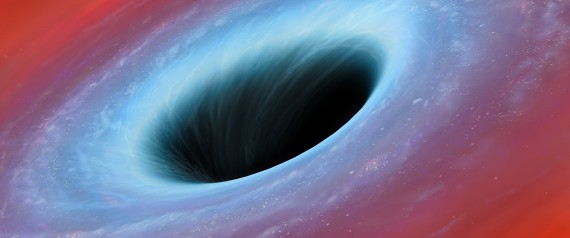
\includegraphics[width=0.7\textwidth]{n-117451542-large570}
%%%			\end{center}
%%		\end{figure}
%	\end{frame}
	
	\begin{frame}{Gliederung}
		\tableofcontents
	\end{frame}
	
	\section{Was ist Informationsentropie?}
	\begin{frame}{Informationsentropie}
		\begin{block}{}
			Die Entropie zählt wie viele Mikrozustände eines Systems einen Makrozustand bilden. 
			
			Beispiel: Wurf von zwei W6-Würfeln.
		\end{block}
		
		\begin{block}{}<2->
		Wie viele Ja-Nein-Fragen muss man beantworten, um das Ergebnis zu bekommen?
		(Im Falle von genau zwei möglichen Ausgängen.)
		Beispiel: Münzwurf hat die Informationsentropie von 1 Bit.	
		\end{block}
%		\hfill
		\begin{figure} [h] 
			\begin{center}
				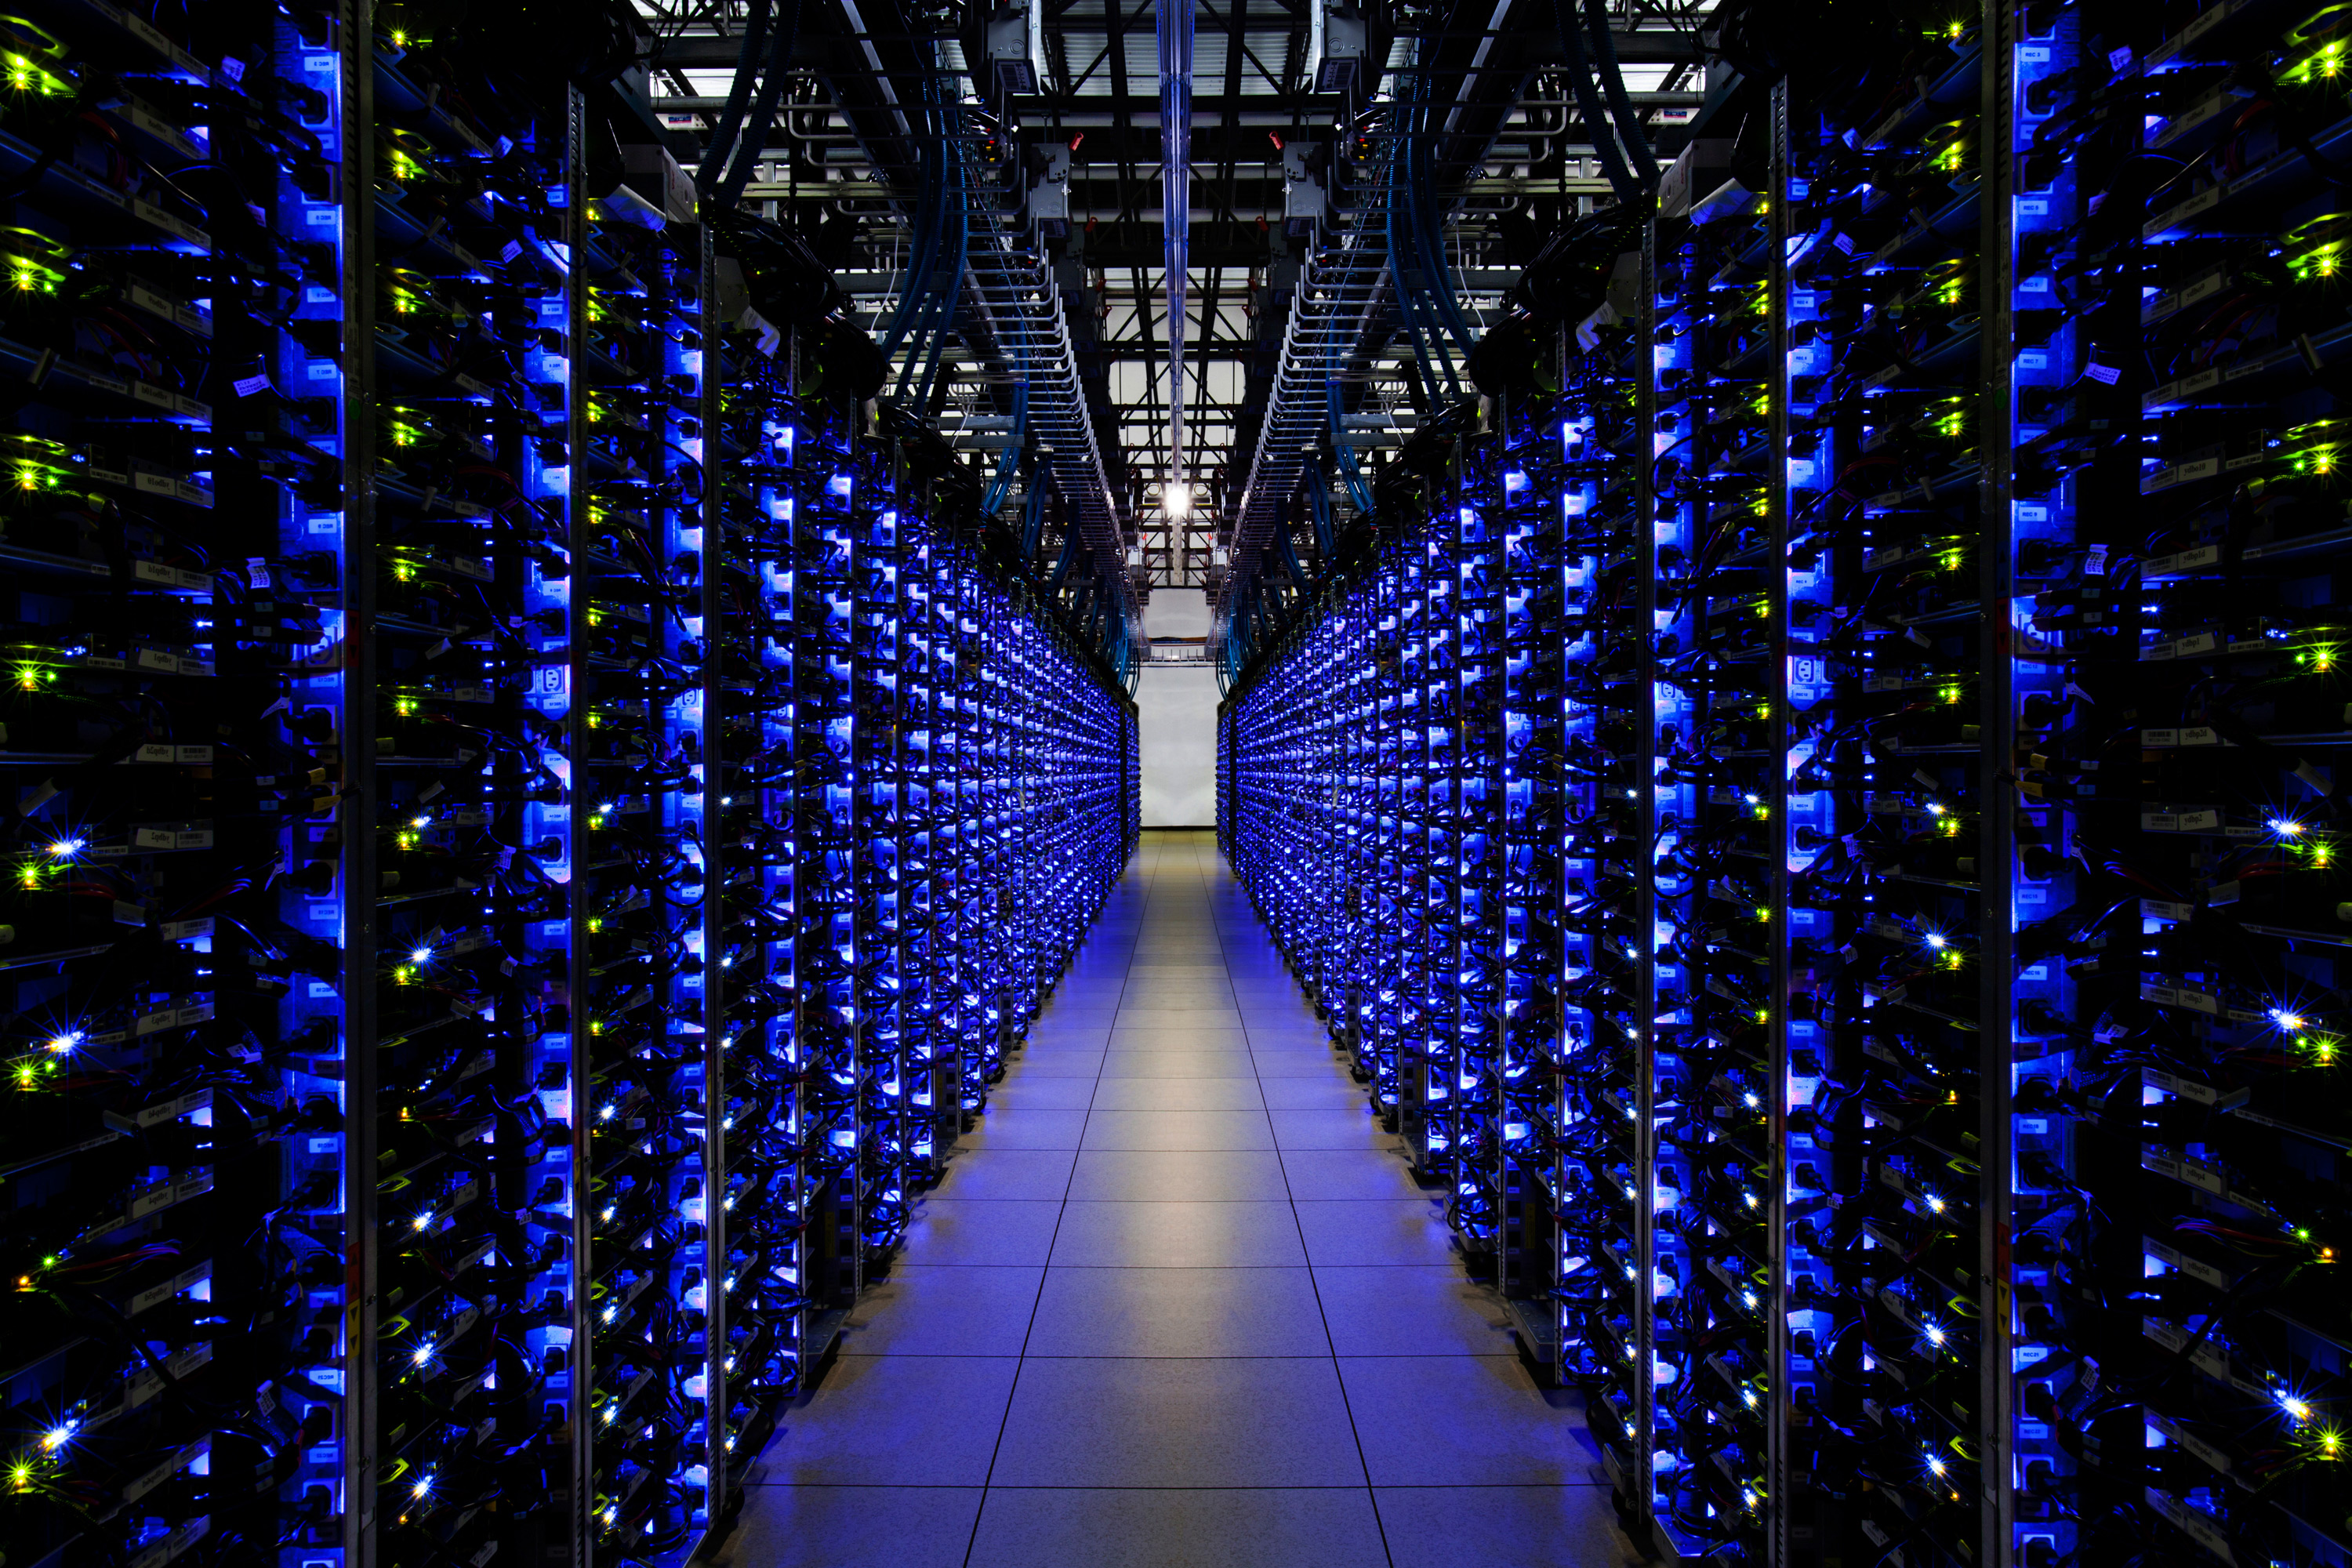
\includegraphics[width=0.5\textwidth]{Server}
			\end{center}
		\end{figure} 	 	%http://www.google.com/about/datacenters/gallery/images/_3000/IDI_018.jpg	
		\hfill
	\end{frame}
	
	\section{Die drei Hauptsätze}
	\begin{frame}{Der Nullte Hauptsatz der Thermodynamik}
		\begin{center}
			\Large{Die Hawkingstrahlung} 
		\end{center}
		\begin{figure} [h] 
			\begin{center}
				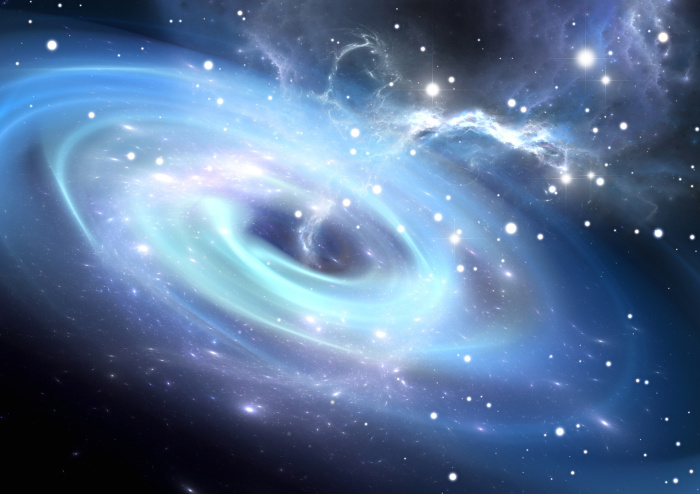
\includegraphics[width=0.5\textwidth]{Hawkingstrahlung}
			\end{center}
		\end{figure} %http://www.spektrum.de/fm/912/thumbnails/SchwarzesLoch_fotolia64583984_PeterJurik.1584161.jpg.1584174.jpg		
	\end{frame}
	
	\begin{frame}{Der Nullte Hauptsatz der Thermodynamik}	
		\begin{figure} [h] 
			\begin{center}
				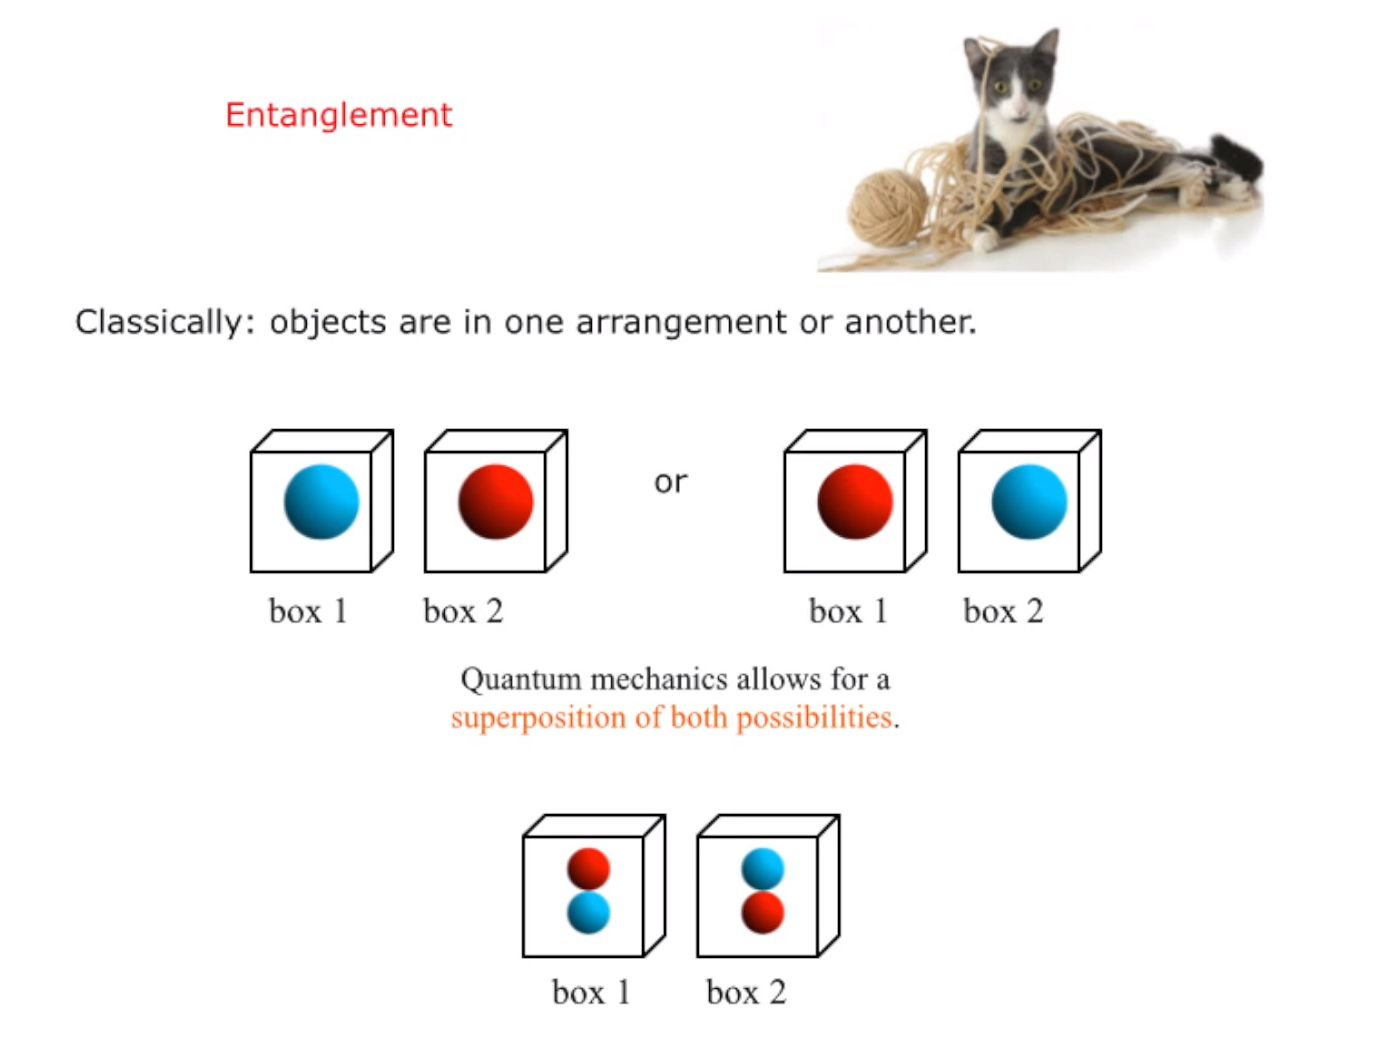
\includegraphics[width=0.8\textwidth]{entanglement}
			\end{center}
		\end{figure} 	%https://www.youtube.com/watch?v=_8bhtEgB8Mo&feature=youtu.be
	\end{frame}
	\begin{frame}{Der Nullte Hauptsatz der Thermodynamik}
		\begin{center}
			\Large{Die Hawkingstrahlung} 
		\end{center}
		\begin{figure} [h] 
			\begin{center}
				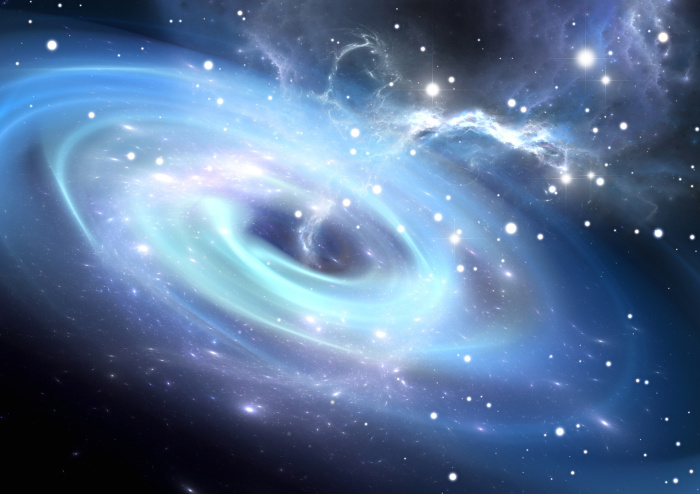
\includegraphics[width=0.5\textwidth]{Hawkingstrahlung}
			\end{center}
		\end{figure} %http://www.spektrum.de/fm/912/thumbnails/SchwarzesLoch_fotolia64583984_PeterJurik.1584161.jpg.1584174.jpg	
		\begin{block}{}
			Nullter Hauptsatz besagt nun, dass genauso viel Wärmestrahlung aufgenommen werden muss, wie abgestrahlt wird 
		
			$\Rightarrow$ Beschleunigung an der Oberfläche	
		\end{block}
	\end{frame}
	
	
	\begin{frame}{Der Erste Hauptsatz der Thermodynamik}
		Der erste Hauptsatz der Thermodynamik besagt Energieerhaltung:
		\begin{align*}
		\Delta U = \Delta Q + \Delta W
		\end{align*}
		\begin{columns}
			\begin{column}{6cm}<2->
				Umgeschrieben:
					\begin{align*}
					\diff E = T\diff S + \diff W
					\end{align*}
				Analogie zu schwarzen Löchern mit Hilfe von Kerr-Neumann-Metrik und geschickt gewählten Koordinaten
			\end{column}
			\begin{column}{4.5cm}<2->
%				\begin{minipage}[l]{0.4\textwidth}
					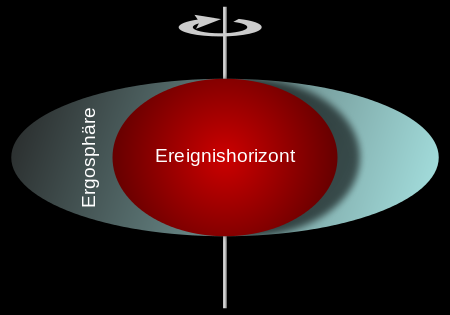
\includegraphics[width=\textwidth]{Kerr-Neumann}
%				\end{minipage} %https://de.wikipedia.org/wiki/Kerr-Metrik (12.01.20016)
				\vfill
			\end{column}
		\end{columns}
	\vfill
		\begin{block}{}<3->
		\underline{Ergebnis:}~~~~
%			\begin{align*}
			\centering{$\diff (Mc^2) = \frac{\kappa}{8 \pi G} \diff A + \Omega \diff J - \Phi \diff q$}
%			\end{align*} 
		\end{block}	 		
	\end{frame}	

	\begin{frame}{Der Zweite Hauptsatz der Thermodynamik}
		\begin{block}{}
		Es gilt Proportionalität der Oberfläche des schwarzen Lochs zur Masse, elektrischer Ladung und Drehmoment.
		\end{block}
		\vfill
		\begin{columns}
			\begin{column}{\textwidth}<2->
			Durch die Hawkingtemperatur und die Definition von Temperatur in der Thermodynamik
			\begin{align*}
				\frac{\diff S}{\diff E} &= \frac{1}{T},&
				T_{\text{Hawking}} &= \frac{\hbar c^3}{8 \pi G M}
			\end{align*}
			und durch Ersetzen von $E = Mc^2$, erhalten wir
			\end{column}
		\end{columns} 
		\begin{columns}
			\begin{column}{\textwidth}<3->
			\begin{align*}
				S_{BH} &= \frac{c^3 A}{4 G \hbar} = \frac{A}{4 \ell_{\mathrm{P}}^2} 
			\end{align*}
			\end{column}
		\end{columns}
	\end{frame}
	
	\begin{frame}{Der Zweite Hauptsatz der Thermodynamik}
		\begin{columns}
			\begin{column}[c]{0.45\textwidth}<2->
				\centering{Holographisches Prinzip}
			\end{column}
			\begin{column}[c]{0.45\textwidth}<3->
				\centering{$M_3 > M_2 + M_1$}
			\end{column}
		\end{columns}
		\vspace{0.3cm}
		\begin{columns}
			\begin{column}[c]{0.45\textwidth}<2->
				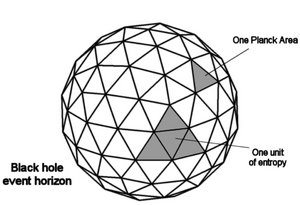
\includegraphics[width=\textwidth]{BHentropy1}
			\end{column}
			\begin{column}[c]{0.45\textwidth}<3->
				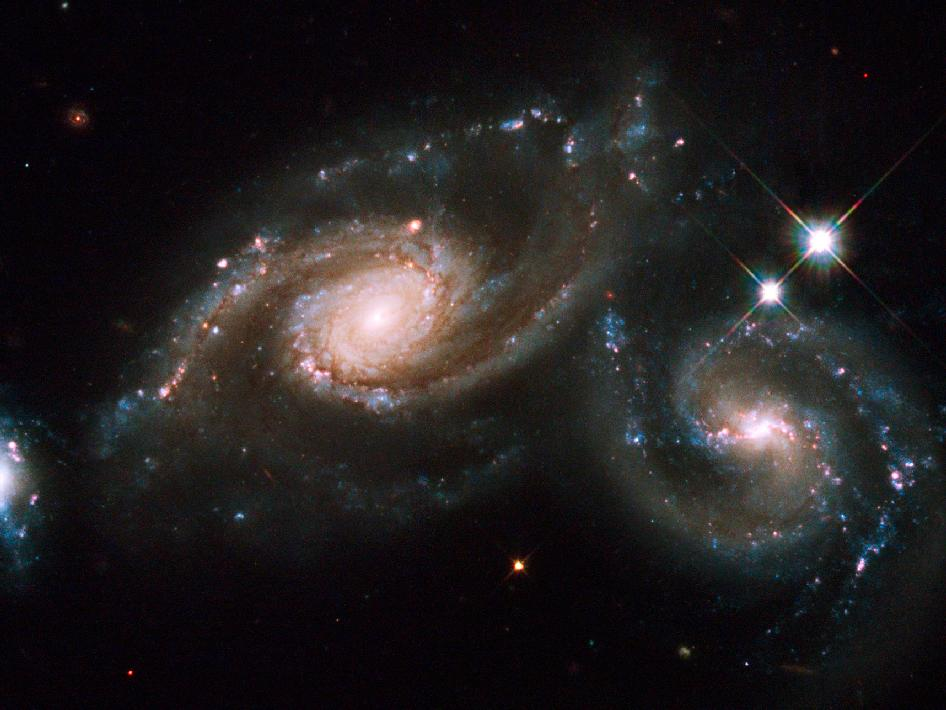
\includegraphics[width=\textwidth]{kollidierendeSHs}
			\end{column}
		\end{columns}
%		\begin{figure} [h] 
%			\begin{center}
%				\movie[externalviewer]{vlc}{earthpointofview_wmv}
%			\end{center}
%		\end{figure}
	\end{frame} %quelle: http://www.nasa.gov/mission_pages/hubble/multimedia/arp274_prt.htm
	
	\section{Verdampfung}
	\begin{frame}{Verdampfung/Evaporation}	
	Man findet: $\frac{\diff E}{\diff t} \approx \frac{C}{r_s^2}$
	$\Rightarrow$ Analogie zum Stefan-Boltzmann Gesetz:
		\begin{align*}
			\frac{\diff E}{\diff A \diff t} = \sigma T^4
		\end{align*}
	\begin{columns}	
		\begin{column}{0.5\textwidth}	
		Für die Masse:
			\begin{align*}
				\frac{\diff M}{\diff t} = - \frac{C}{(GM)^2}
			\end{align*}
		Daraus ergibt sich:
			\begin{align*}
				t_{\text{evap}} \sim G^2 M^3
			\end{align*} 
		\end{column}
		\begin{column}{0.5\textwidth}
			\begin{figure} [h] 
					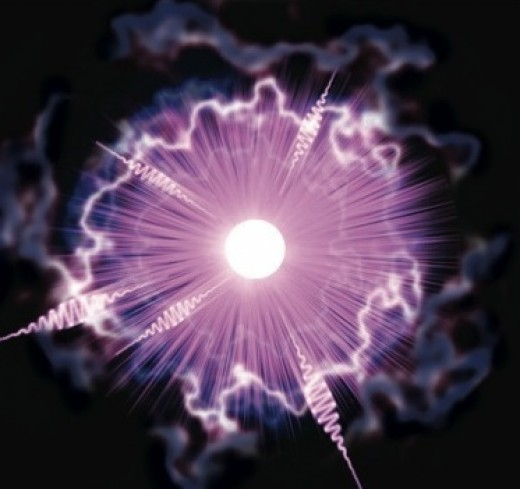
\includegraphics[width=0.8\textwidth]{evaporation}
			\end{figure}
		 %http://hubpages.com/education/Hawking-Radiation-and-Evaporating-Black-Holes#slide4018139
		 \end{column}
	\end{columns}
	\end{frame}
	
	\section{Weitere Betrachtung}
	\begin{frame}{Weitere Betrachtung}
		\begin{block}{Wirkungsintegrale}
		Die Zustandssumme: 
			\begin{align*}
			Z = \int \diff [\Phi] \exp \left(- \frac{I_E}{\hbar}\right) 
			\simeq \exp \left(- \frac{I_{E,B}}{\hbar}\right)
			\end{align*}
		\end{block}
		\begin{block}{Loop Quantum Gravity}<2->
			\begin{columns}
				\begin{column}[c]{0.45\textwidth}
					Es existieren schwarze und weiße Löcher, aber keine Singularität.
				\end{column}
				\begin{column}[c]{0.45\textwidth}
					\hfill
					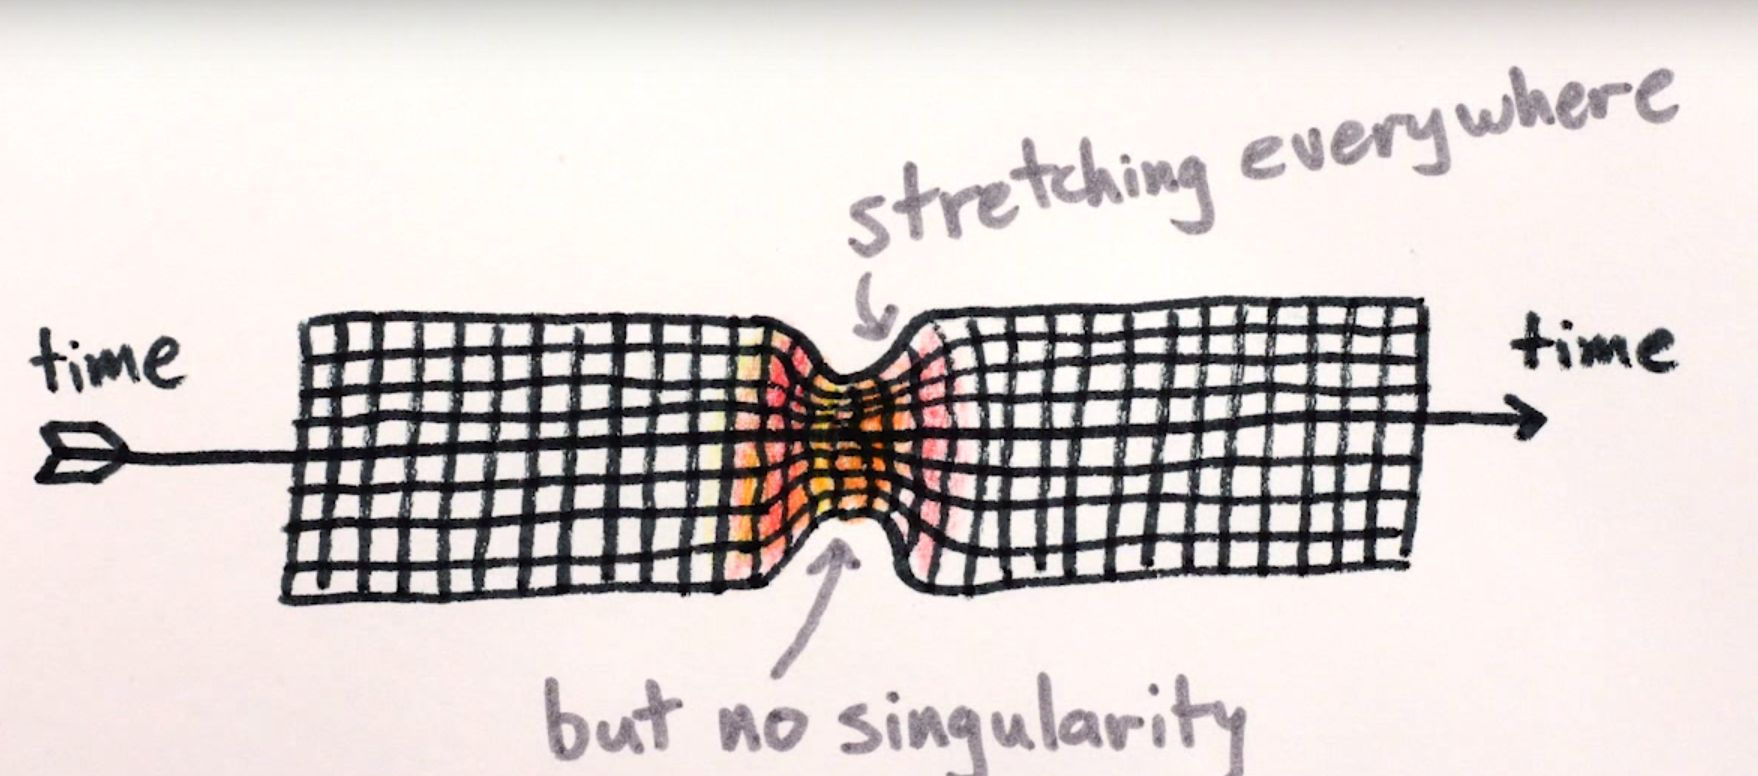
\includegraphics[width=\textwidth]{bounce1}
				\end{column} % http://pics-about-space.com/black-matter-black-holes?p=2#
			\end{columns}
		\end{block} 
%		\begin{figure} [h] 
%			\begin{center}
%				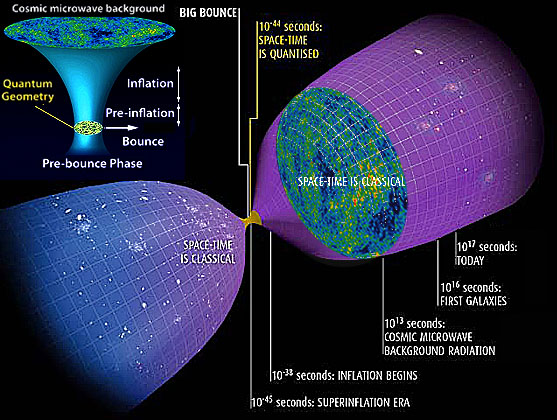
\includegraphics[width=0.5\textwidth]{bounce}
%			\end{center}
%		\end{figure} 
	\end{frame}	
	
	\begin{frame}
		\begin{minipage}[c]{\textwidth}
			\huge{Vielen Dank für Eure Aufmerksamkeit!}
		\end{minipage}	
		\begin{figure} [h] 
			\begin{center}
				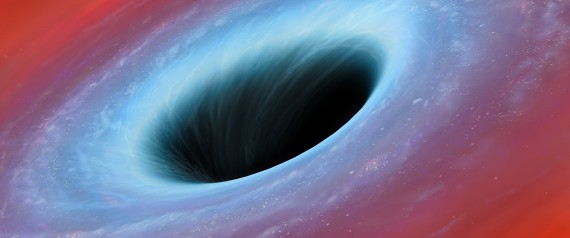
\includegraphics[width=0.7\textwidth]{n-117451542-large570}
			\end{center}
		\end{figure}	
	\end{frame}
\end{document}